\documentclass[a5paper, 12pt]{book}
\usepackage{geometry}
\usepackage [ngerman] {babel}
%enumerate kann man dann anpassen
\usepackage{enumerate}
%Um Bilder einzufügen
\usepackage{graphicx}
%um subfigures zu erstellen, damit ich mehrere bilder zu einer figure zusammenfügen kann
\usepackage{caption}
\usepackage{subcaption}
\usepackage{hyperref}

\usepackage{anyfontsize}
\usepackage{textcomp}
%SubSubsections werden gezählt
\setcounter{tocdepth}{3}
\setcounter{secnumdepth}{3}

\geometry{a5paper, total = {4in,5in}}

\newcommand{\neueregel}{
\noindent Regel, die geändert oder hinzugefügt werden soll:

\vspace{2cm}
\noindent Was soll geändert/hinzugefügt werden?

\vspace{13cm}
Antragsteller:
\newpage
}
\newcommand{\twoemptypages}{
\thispagestyle{plain}
\mbox{}
\newpage
\thispagestyle{plain}
\mbox{}
\newpage
}




\begin {document}
\renewcommand{\listfigurename}{Abbildungs- verzeichnis}
\pagenumbering{gobble}
\newgeometry{top=6cm, total = {4in,5in}}
\begin{titlepage}
\begin{center}
{\fontsize{40}{48}\selectfont \textbf{Wal-BGB}\par}

\begin{large}
\vspace{0.3cm}
Das große Bierponggesetzbuch\\
\vspace{1cm}
Smion Schweiger Schweiger\\
\vspace{1cm}
3. Auflage, September 2025
\end{large}
\end{center}
\vspace{6cm}
Herstellung und Verlag: SBG CopyShop an der Uni
\end{titlepage}

\begin{center}
\vspace*{2.5cm}
\scalebox{3.5}{\S 420}
\par
\smallskip
\large{Im Zweifel hat immer ein Wal-WG\texttrademark-Mitglied Recht.}
\end{center}
\restoregeometry
\pagebreak
\begin{Large} \textbf{Vorwort\\}
\end{Large}
Dieses Buch ist entstanden, um den Bierpong-Spielen in der Wal-WG eine stabile Regelgrundlage zu geben und sämtliche Unklarheiten aus der Welt zu schaffen. Da der Autor allerdings kein Jurist, sondern nur lausiger Lehramtler ist, werden sich sicherlich noch allerlei Fehler finden, auch nachdem für die 3. Auflage schon einiges ausgebessert worden ist. Extra dafür gibt es Platz im Anhang, wo Anmerkungen zu Lücken im Regelwerk, Logikfehlern o.ä. gemacht werden können. Gerne sind auch andere Anmerkungen und Wünsche gesehen, solange sie irgendetwas mit Bierpong zu tun haben.\\
Es gibt eine große Regeländerung für die dritte Auflage: Man kann sich jetzt am Anfang des Spiels entscheiden, ob man bei geraden oder ungeraden Bechern umstellen will.Eine weitere gänzlich neue Regel ist es, dass man jetzt außer onFire auch onIce sein kann. Außerdem gab es viele kleine Anpassungen, die Feinheiten bei der Auslegung verbessern.
In der dritten Auflage wurden einige Änderungen an der Form vorgenommen. Die beiden wichtigsten sind die Verwendung des generischen Femininums und das \texttrademark. Eine vollständige Auflistung aller Änderungen gibt es bei den Patchnotes (\ref{chap:patchnotes}).\\
Gedankt sei allen Leuten, die in der Wal-WG\texttrademark schon Bierpongmatches bestritten haben, und damit den Grundstein für die Entwicklung des Regelwerks gelegt haben. Außerdem geht Dank an Vinne, der die ganzen hübschen Abbildungen und das Cover für die dritte Auflage erstellt hat, außerdem Sabrina, für das neue Ablaufdiagramm, sowie an generell alle die sich die Mühe gemacht haben den Spaß Korrektur zu lesen.\\\\
Dank geht auch raus an alle, die Input für nötige Regeländerungen gegeben haben, oder einfach Spiele gespielt haben und damit die bisherigen Auflagen an ihre Grenzen gebracht haben.
Ich hoffe, dass das doch recht formelle Regelwerk das Spiel jetzt nicht verkopft, eigentlich wollen wir ja doch alle nur n Rausch.

\tableofcontents
\cleardoublepage
\pagenumbering{arabic}
\part {Regeln}\label{part:regeln}
\chapter*{Regelverstoß}\label{chap:regelverstoß}
Im Weiteren Verlauf des Regelwerks wird beschrieben, wie genau ein Bierpong Spiel in der Wal-WG\texttrademark abläuft. Teilweise werden konkrete Strafen genannt, wenn sich an bestimmte Regeln nicht gehalten wird. Für alle anderen Regeln und Prinzipien gilt, dass ein Verstoß unsportlich ist und jederzeit zur Disqualifikation durch ein Wal-WG\texttrademark Mitglied führen kann. 

\chapter{Definitionen} \label{chap:definitionen}
\section{Becher trinken} \label{sec:bechertrinken}
Wenn die Rede davon ist, dass Becher getrunken werden müssen, dann muss eine Spielerin des Teams, das trinken muss, entweder den Becher trinken/den Inhalt in den aktuell getrunken werdenden Becher füllen/das Äquivalent für den Becher aus einem anderen Gefäß trinken (nur wenn das von vornherein abgemacht war und im Becher Wasser war). Außerdem muss der getrunkene Becher an den Tischrand gestellt werden. Sobald ein Team anfängt, den Becher zu trinken, zählt er nicht mehr zu ihren Bechern. Als vollständig getrunken zählt der Becher, wenn weniger als 10 ml Flüssigkeit sich in ihm befinden.
\section{Standardwurf}\label{sec:standardwurf} 
Eine Spielerin steht auf der eigenen Seite des Tisches. Es darf sich nicht irgendwo erhöht hingestellt werden, außer es bringt keinen Vorteil, weil es zum Beispiel deutlich weiter hinten ist. 
\section{Trickshot}\label{sec:trickshot}
Ein Trickshot muss auf irgendeine Art und Weise anders geworfen werden als ein Standardwurf, oder auf kreative Art und Weise in Richtung der gegnerischen Becher befördert werden. Voraussetzung, dass es als Trickshot zählt, ist dass er schwieriger zu treffen ist als ein Standardwurf(z.B über die Wand, rückwärts, Weltraumlaser etc.). Wenn ein Trickshot, nachdem er geworfen wurde, 2- mal auf dem Tisch abprallt, darf er vom Gegnerteam gefangen oder weggeschlagen werden.\\\\
Mit geschlossenen Augen oder der schwachen Hand zu werfen ist KEIN Trickshot, außer dies wird explizit so vereinbart.\\\\
Außerdem zählen folgende Varianten als Trickshot:
\begin{enumerate}[(1)]
    \item Gastwurf: eine Zuschauerin darf den Wurf ausführen. Dieser ist es dann erlaubt einen Standardwurf durchzuführen. Da der Standardwurf einfacher zu treffen ist, als ein Trickshot, gilt es als unsportlich, deutlich mehr Gastwürfe als das andere Team durchzuführen (selbstverständlich in Relation zu der gesamten Anzahl an Trickshots pro Team gesehen, nicht absolut).
    \item Ein Standardwurf, bei dem die Werferin komplett nackt ist.
\end{enumerate}

\section{Treffer}\label{sec:treffer}
Ein Becher zählt als getroffen, wenn eine der folgenden Bedingungen eintritt:
\begin{enumerate} [(1)]
    \item Ein gültiger Standardwurf (siehe Abschnitt \ref{sec:standardwurf}) oder Trickshot (siehe Abschnitt \ref{subsub:Trickshotphase}) landet in einem Becher und bleibt dort liegen.\\
    \item Ein Standardwurf (siehe Abschnitt \ref{sec:standardwurf}) oder Trickshot (siehe Abschnitt \ref{subsub:Trickshotphase}) sorgt dafür, dass ein Becher umfällt und vollständig ausläuft. Als vollständig ausgelaufen zählt der Becher, wenn sich weniger als 10ml noch in dem Becher befinden. Wird er gefangen, oder landet richtig, so dass er nicht vollständig ausläuft wird er an die Position zurückgestellt, an der er stand, unmittelbar bevor er gefallen ist. \\
Mit Absicht so zu werfen, dass die Becher umfallen ist unsportliches Verhalten und wird in der Wal-WG\texttrademark nicht toleriert!
\item Ein Team schusselt auf irgendeine Art und Weise unabsichtlich den Ball in einen eigenen Becher hinein. Dies zählt als Treffer für die Gegner, allerdings nicht für eine bestimmte Spielerin.

\item  Eine Spielerin eines Teams schmeißt außversehen einen eigenen Becher um, und es verbleiben weniger als 10ml in dem Becher. Dies zählt als Treffer für die Gegner, allerdings nicht für eine bestimmte Spielerin. 
\end{enumerate}
Ein nach diesen Bedingungen getroffener Becher zählt immer auch als \textit{gehitted}. Der Begriff \textit{gehitted} wird im Regelwerk noch einige male verwendet und ist klar abzugrenzen von einem Treffer. Zum Beispiel bei der Bombe (siehe Abschnitt \ref{sec:bombe}) kann man einen Becher als gehitted markieren ohne ihn zu treffen. 
\chapter{Spielaufbau} \label{chap:spielaufbau}
Auf der nächsten Seite wird der grundlegende Aufbau eines jeden Bierpong-Spiels in der Wal-WG\texttrademark dargestellt. Als Tisch ist der hauseigene Biertisch zu verwenden und traditionell wird im Bad gespielt. Zum Werfen sind nur Tischtennis Trainings- oder Spielbälle zu verwenden. Billige, eindrückbare whacke Bierpong Tedi Bälle o.ä. sind strikt verboten. Es wird mit 0,4 - 0,5 Liter fassenden Plastikbechern gespielt. Außerdem muss für ein Spiel die Badtür ausgehängt werden. \\
In der folgenden Abbildung ist ein reguläres Spiel mit 2 Bier (je 0,5 Liter) pro Team abgebildet. Es sind auch alternative Varianten möglich, bei denen die Becher mit Wein o.ä. gefüllt werden. Theoretisch ist es auch erlaubt die Becher mit Wasser zu füllen und etwas anderes oder nichts zu trinken, dies ist aber nicht gerne gesehen. Jegliche Abweichung von der Standardbefüllung muss vom Gegnerteam bewilligt werden.

\begin{figure}
    \centering
    \begin{subfigure}[h]{0.69\textwidth}
    \centering
    \includegraphics[width=\textwidth]{beerpongregeln_ohne_legende.png}
    \caption{Aufbau}
    \end{subfigure}
    \hfill
   \begin{subfigure}[h]{0.29\textwidth}
   \centering
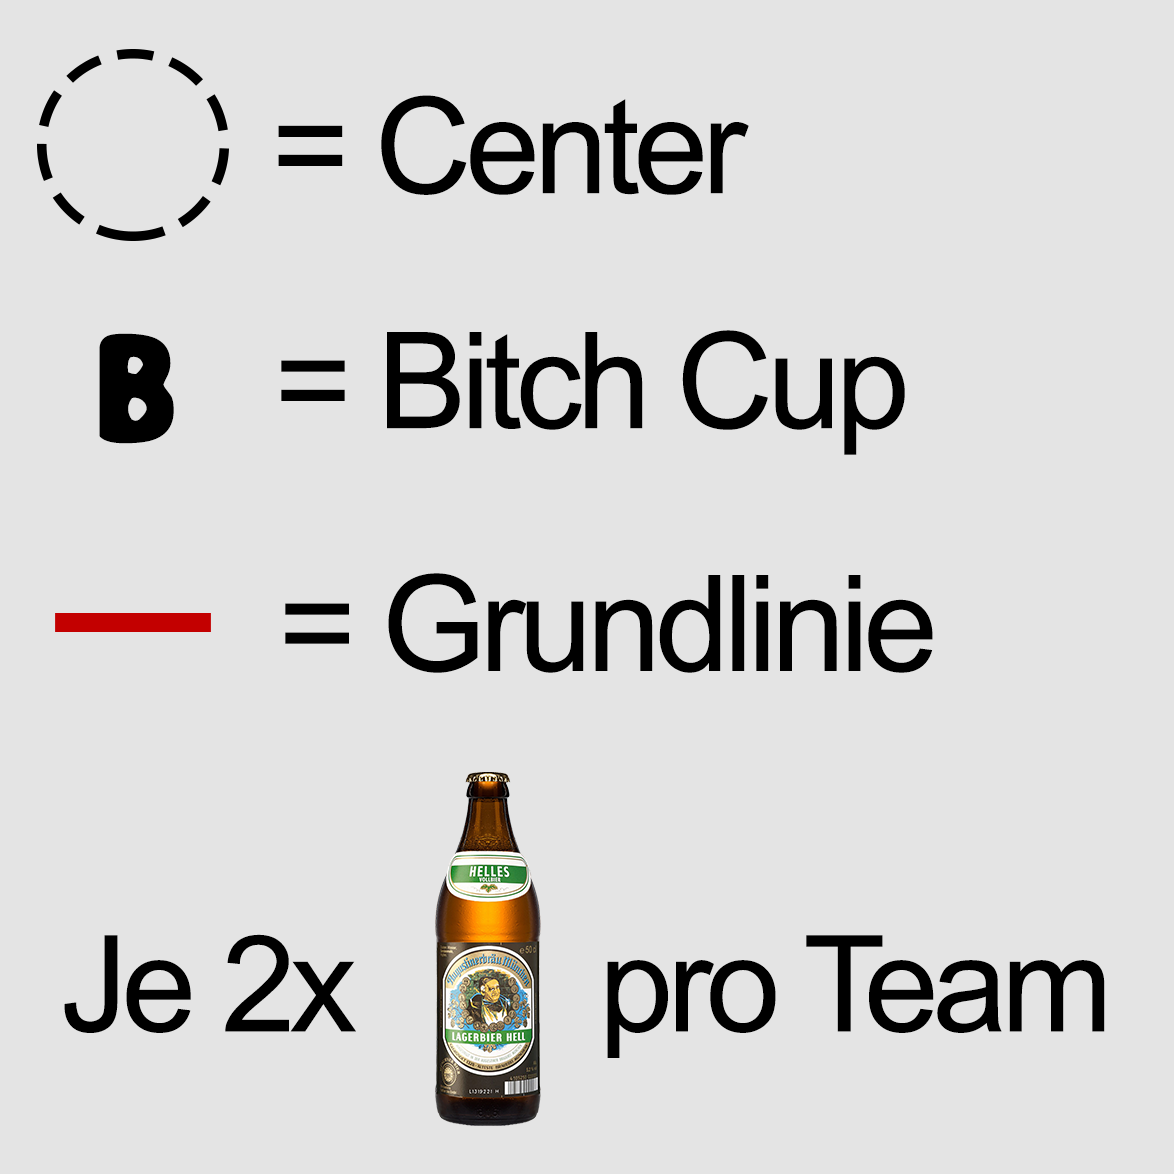
\includegraphics[width=\textwidth]{legende.png}
\caption{Legende}
   \end{subfigure}
    \caption{Spielaufbau}
    \label{fig:spielaufbau}
\end{figure}

\chapter{Spielablauf}\label{chap:spielablauf}
\section{Skizze des Spielablaufs}\label{sec:skizze des spielablaufs}
Auf der nächsten Seite wird der grobe Ablauf eines jeden Bierpong-spiels schematisch dargestellt. Genauere Erklärungen zu den einzelnen Phasen folgen im Rest des Kapitels.

\begin{figure} 
    \centering
    \hspace*{-1.5cm}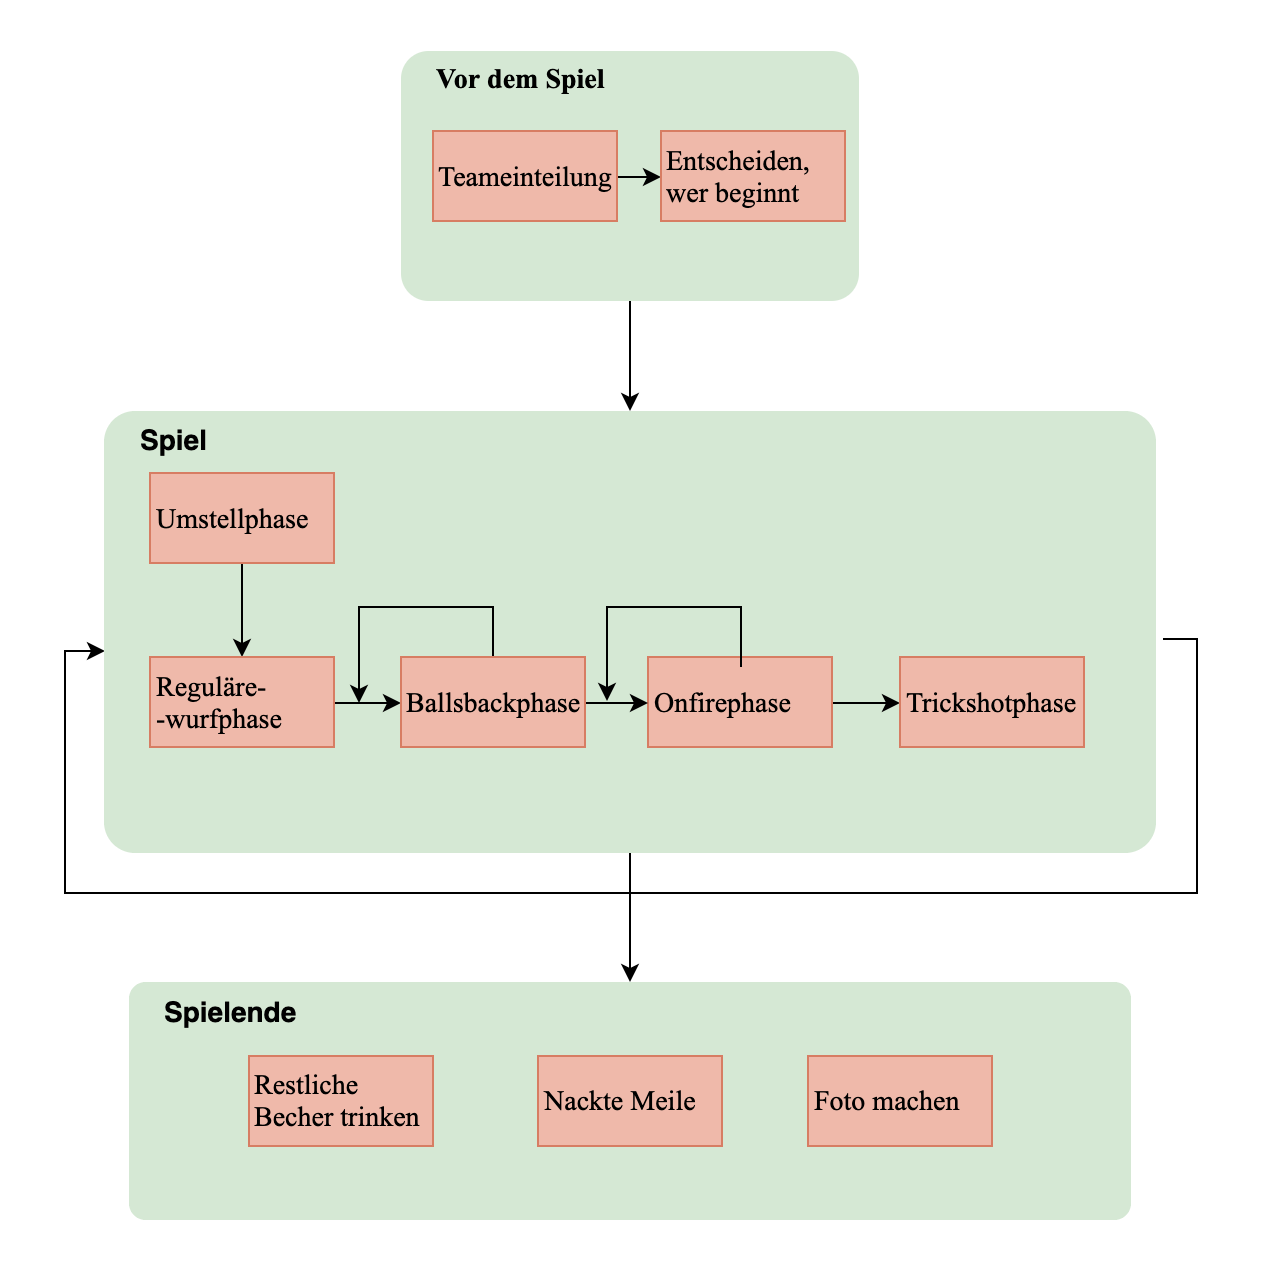
\includegraphics[scale = 0.27]{Bierpongflowneu.png}
    \caption{Spielverlaufsskizze}
    \label{fig:bierpongflow}
\end{figure}

\section{Genaue Regelungen}\label{sec:genaue regelungen}
\subsection{Vor dem Spiel}\label{sub:vor dem spiel}
\subsubsection{Teameinteilung}\label{subsubsec:teameinteilung}
Es finden sich vier Leute ein, die spielen wollen. Damit sie tatsächlich spielen dürfen müssen sie das mit allen anderen, die gerade auch spielen wollen, abklären. Dann teilen sie sich in zweier Teams ein und einigen sich auf eine ihnen frei gestellte Art, wer auf welcher Seite spielt. \\
Es ist auch das Spiel mit einer beliebigen Anzahl an Leuten pro Team möglich. Die Teamgrößen müssen auch nicht identisch sein. Bei einer anderen Teamgröße ändert sich aber am Spiel prinzipiell nichts, es wird trotzdem mit zwei Bällen gespielt, jedes Team hat immer gleich viele Würfe, wie es mit zwei Spielerinnen hätte. Nur wechseln sich die Spielerinnen eines Teams dann so ab, dass sie ähnlich oft werfen.
\subsubsection{Seiteneinteilung}\label{subsub:seiteneinteilung}
Es ist den Spielenden freigestellt, wie sie entscheiden, wer auf welcher Seite spielt. Kommt allerdings keine Einigung zustande, wird eine Runde Schnick Schnack Schnuck ohne Brunnen gespielt.
\subsubsection{Gerade oder Ungerade}\label{subsub:geradeoderungerade}
Jedes Team muss sich jetzt entscheiden, ob es in diesem Spiel bei einer geraden oder bei einer ungeraden Becheranzahl stellen will. Dies wird dann mithilfe der Vorrichtung am Tisch markiert. Sollte dieser Schritt vergessen werden gilt die Markierung, die gerade am Tisch hängt.
\subsubsection{Entscheiden, wer anfängt}\label{subsub:entscheidenweranfängt}
Die normale Variante, wie ermittelt wird wer anfängt ist \textit{Eye to Eye}. Wenn sich beide Parteien einig sind kann aber auch auf irgendeine andere Variante ermittelt werden wer anfängt. \\\\
Eye to Eye:\\
Jedes Team bestimmt ein Teammitglied. Die beiden Bestimmten stehen an ihren Seiten des Tisches, schauen sich in die Augen und werfen gleichzeitig. Wenn eine von beiden trifft, dann fängt ihr Team mit dem Spiel an. Wenn keine oder beide treffen, dann werfen die anderen beiden Teammitglieder. Wenn jetzt eine trifft, darf ihr Team anfangen. Wenn keine oder beide treffen, dann spielen die beiden Spielerinnen, die gerade geworfen haben Best-of-one SchnickSchnackSchnuck ohne Brunnen. Das Team der Siegerin darf dann anfangen. \\\\Das Team, das anfangen darf, startet dann mit dem Spiel in der Umstellphase.\\
Wenn sich bei einem der Würfe die Bälle in der Luft treffen müssen die beiden Werferinnen sich küssen.
\subsection{Spiel}\label{sub:spiel}
Das Spiel besteht aus der Umstellphase und 4 Wurfphasen. \\\\
In der Umstellphase kann die Aufstellung der gegnerischen Becher modifiziert werden. \\\\
In einer Wurfphase werden Hits gesammelt. Wenn eine Phase vorbei ist, müssen alle gehitteden Becher getrunken werden. Insbesondere müssen Becher also auch getrunken werden, wenn eine Phase neu gestartet wird (bei BallsBack \ref{subsub:ballsbackphase} und OnFire \ref{subsub:onfirephase} relevant).\\
 Ausnahme ist, wenn der letzte Becher als gehitted zählt, dann werden nach dem Ende der Phase nur alle Becher bis auf den letzten getrunken. Das Team, dass den Becher eigentlich trinken müsste hat dann in seinen nächsten Wurfphasen die Chance auf Redemption. (siehe Abschnitt \ref{sec:redemption})\\\\
Hat ein Team seine Trickshotphase beendet ist eine Runde abgeschlossen und das andere Team startet die nächste Runde mit dessen Umstellphase, außer das Spiel ist vorbei.\\\\


\subsubsection{Umstellphase}\label{subsub:umstellphase}
In der Umstellphase hat das jeweilige Team 2 Optionen:
\begin{enumerate}[(1)]
    \item Umstellen: \\\\
    Jedes Team darf einmal im gesamten Spiel die Becher des Gegnerteams umstellen. Dies geht nur, wenn das Gegnerteam eine gerade/ungerade (am Anfang der Partie für jedes Team individuell festgelegt\ref{subsub:geradeoderungerade}) Anzahl von Bechern hat. Hierfür muss dem Gegnerteam eine Formation genannt werden, die sie stellen sollen. Beim Umstellen muss jede Bechergruppe mindestens einen Kontakt zur Grundlinie haben. Beispiele hierzu in den nachfolgenden Abbildungen.\\\\
Wenn \textit{die Enge Muschi} (siehe Abbildung \ref{fig:enge-Muschi}) gestellt werden soll, muss explizit um \textit{die Enge Muschi} gebeten werden. Bei Beschreibungen wie z.B \textit{die Enge} oder \textit{die offensive Raute}, darf sich das Team, dass seine Becher bewegen soll, taub stellen. \\
\begin{figure} 
    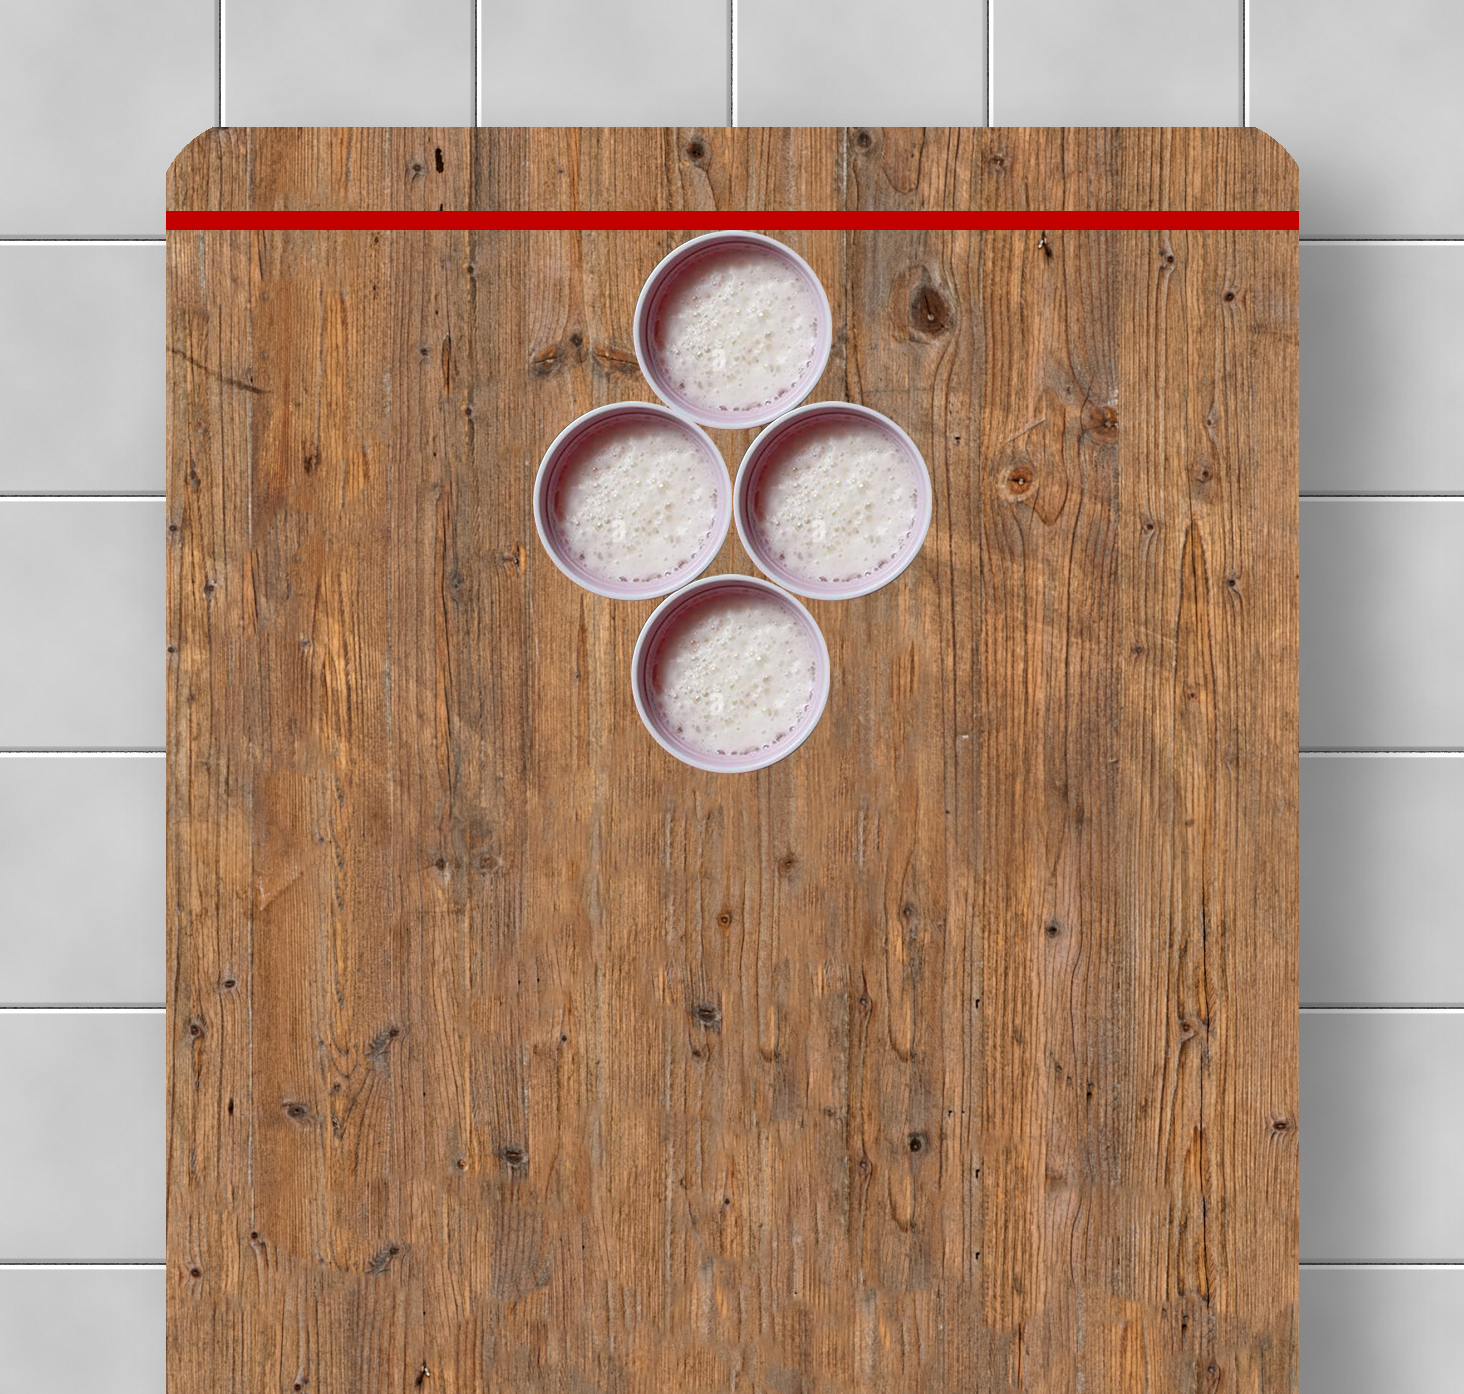
\includegraphics[width=0.434\textwidth]{enge_muschi.png}
    \caption{Die \textit{Enge Muschi}}
    \label{fig:enge-Muschi}
\end{figure}
\begin{figure}[h!]
     \centering
     \begin{subfigure}[b]{0.434\textwidth}
         \centering
         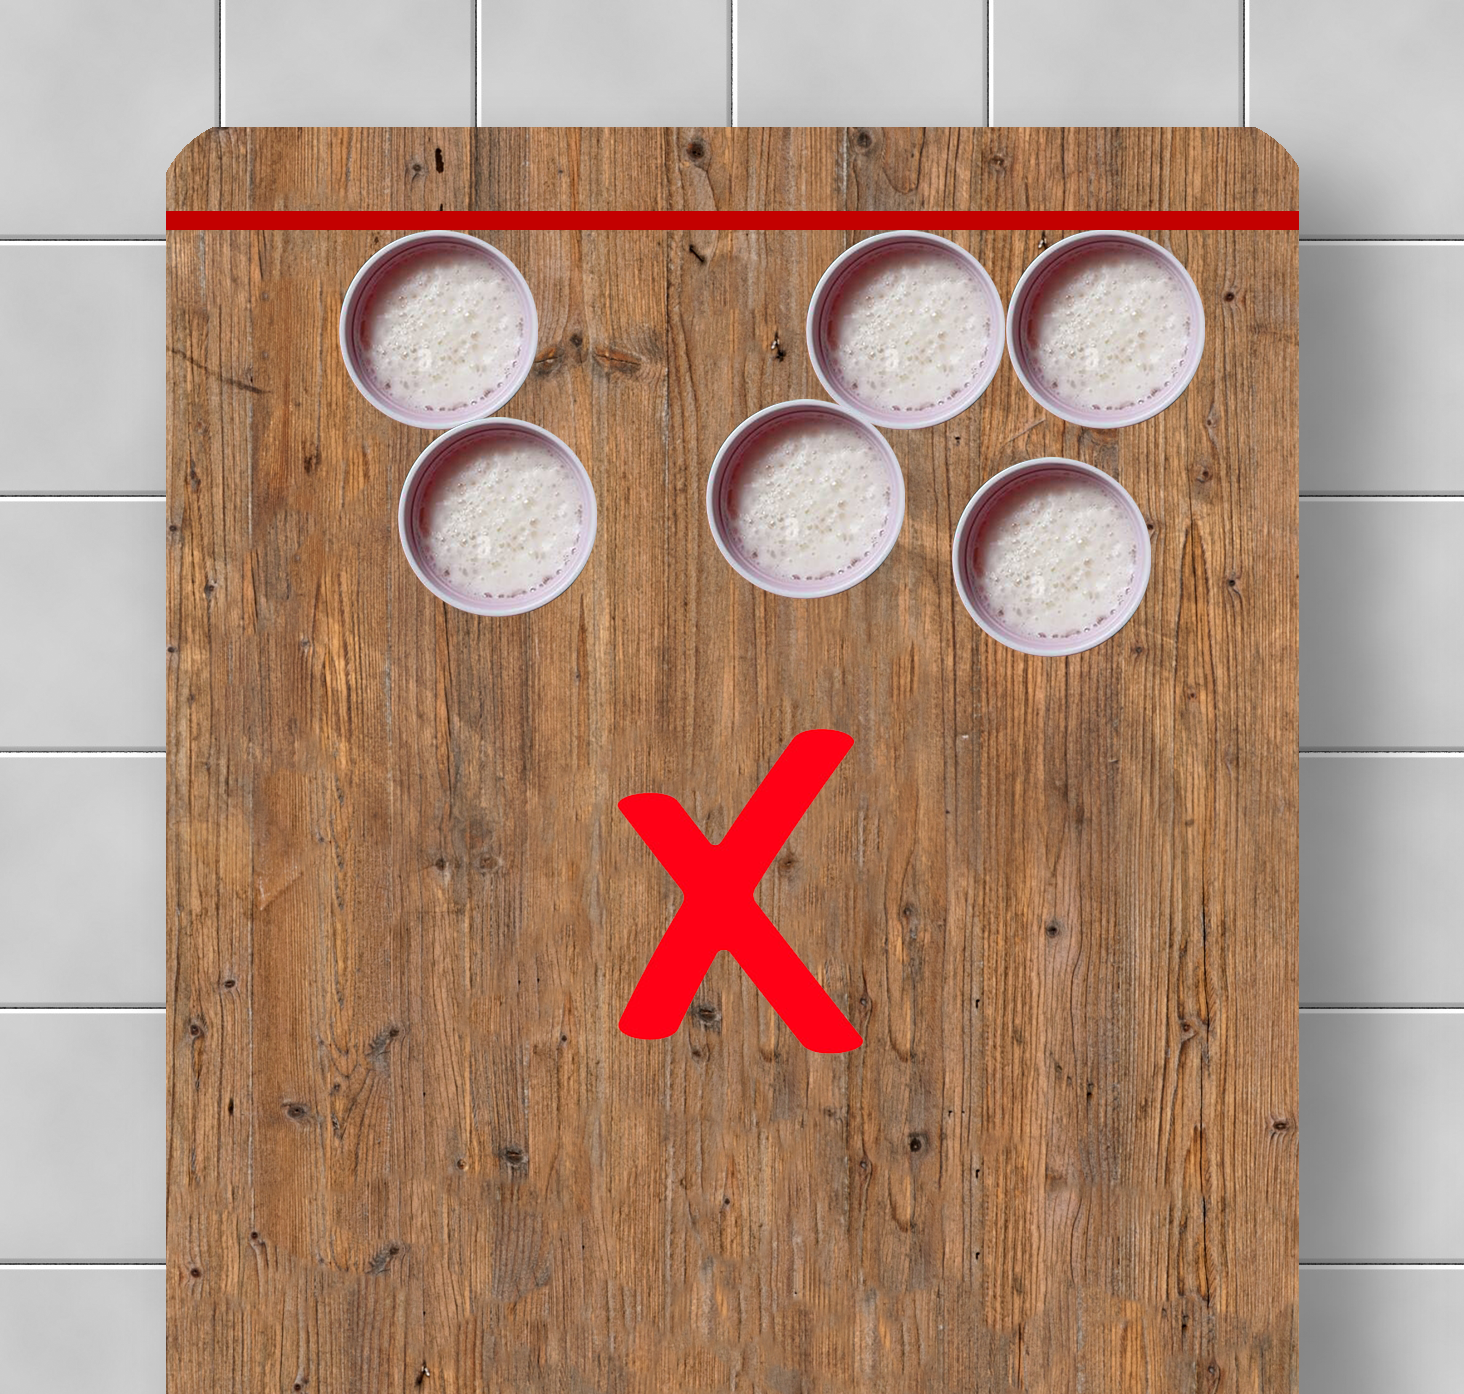
\includegraphics[width=\textwidth]{no1}
         \caption{nicht erlaubte Formation}
    
     \end{subfigure}
     \hfill
     \begin{subfigure}[b]{0.434\textwidth}
         \centering
         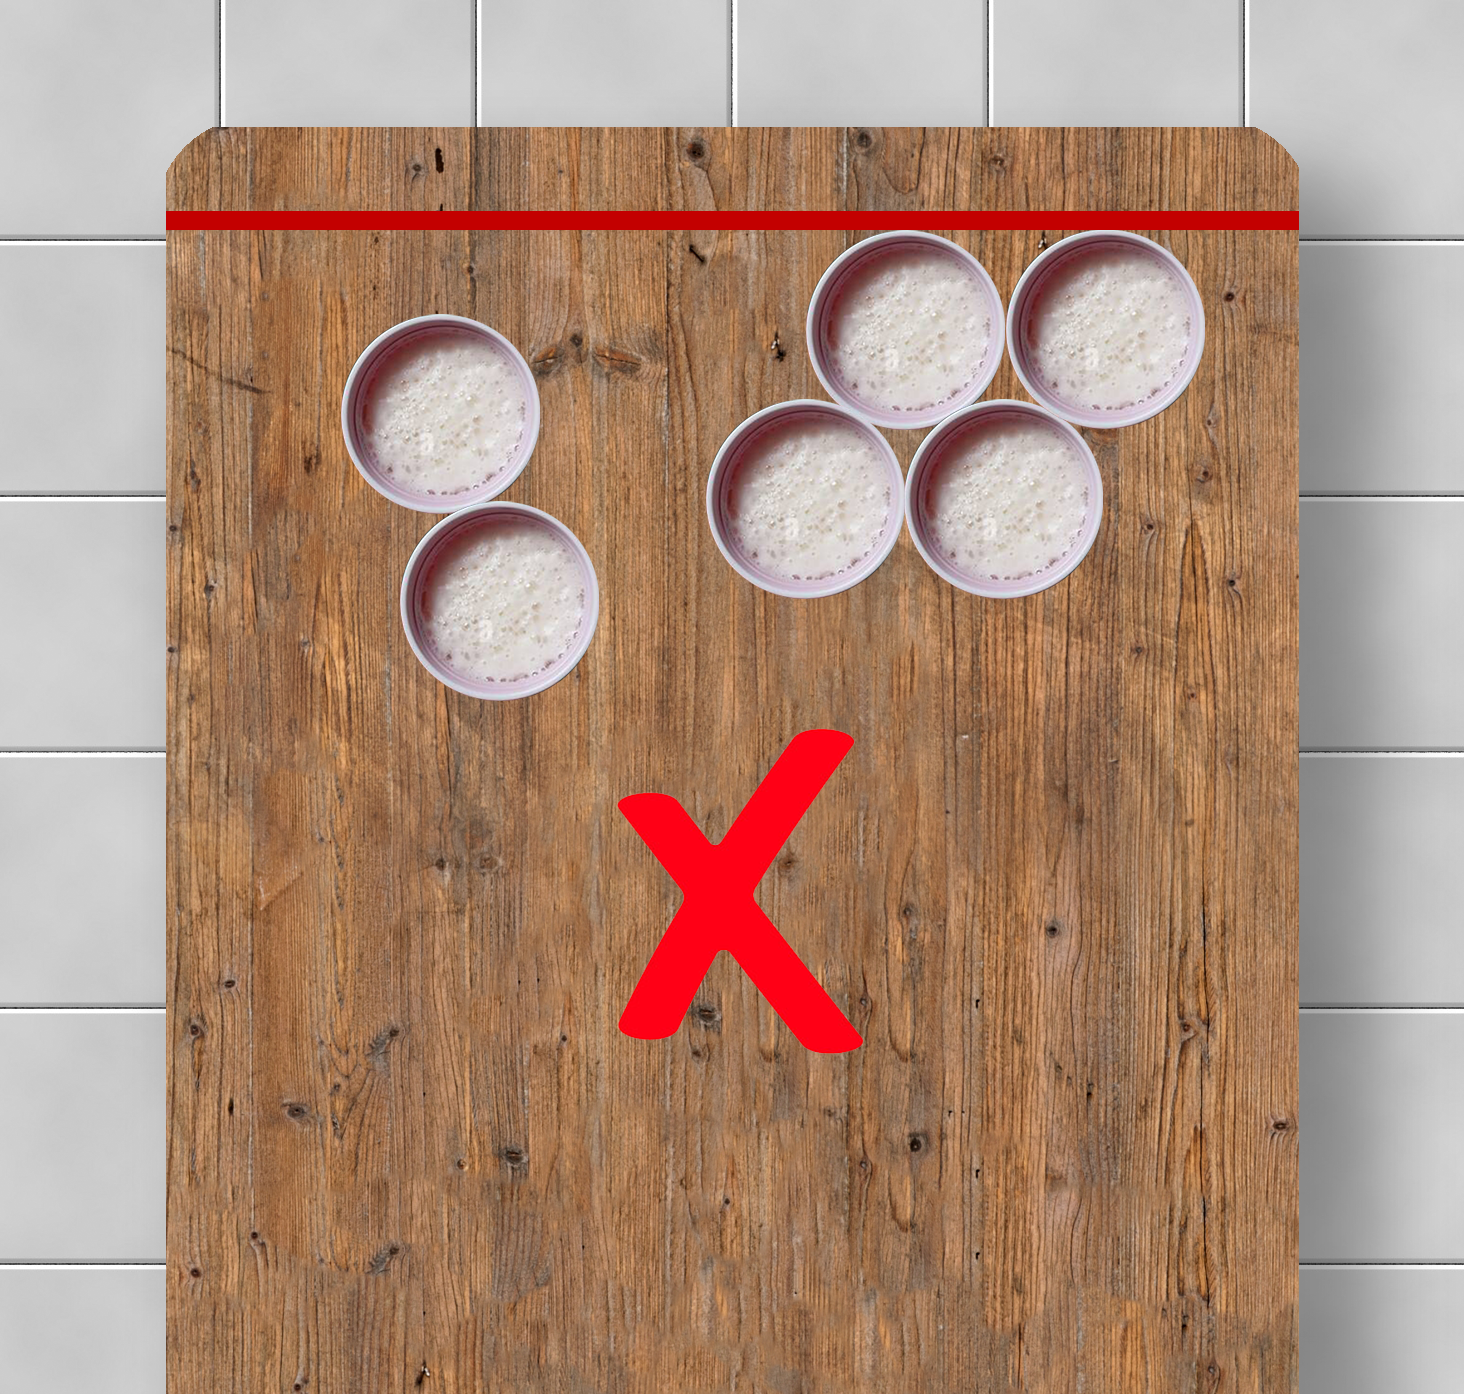
\includegraphics[width=\textwidth]{no2}
         \caption{nicht erlaubte Formation}
     \end{subfigure}
     \hfill
     \begin{subfigure}[b]{0.434\textwidth}
         \centering
         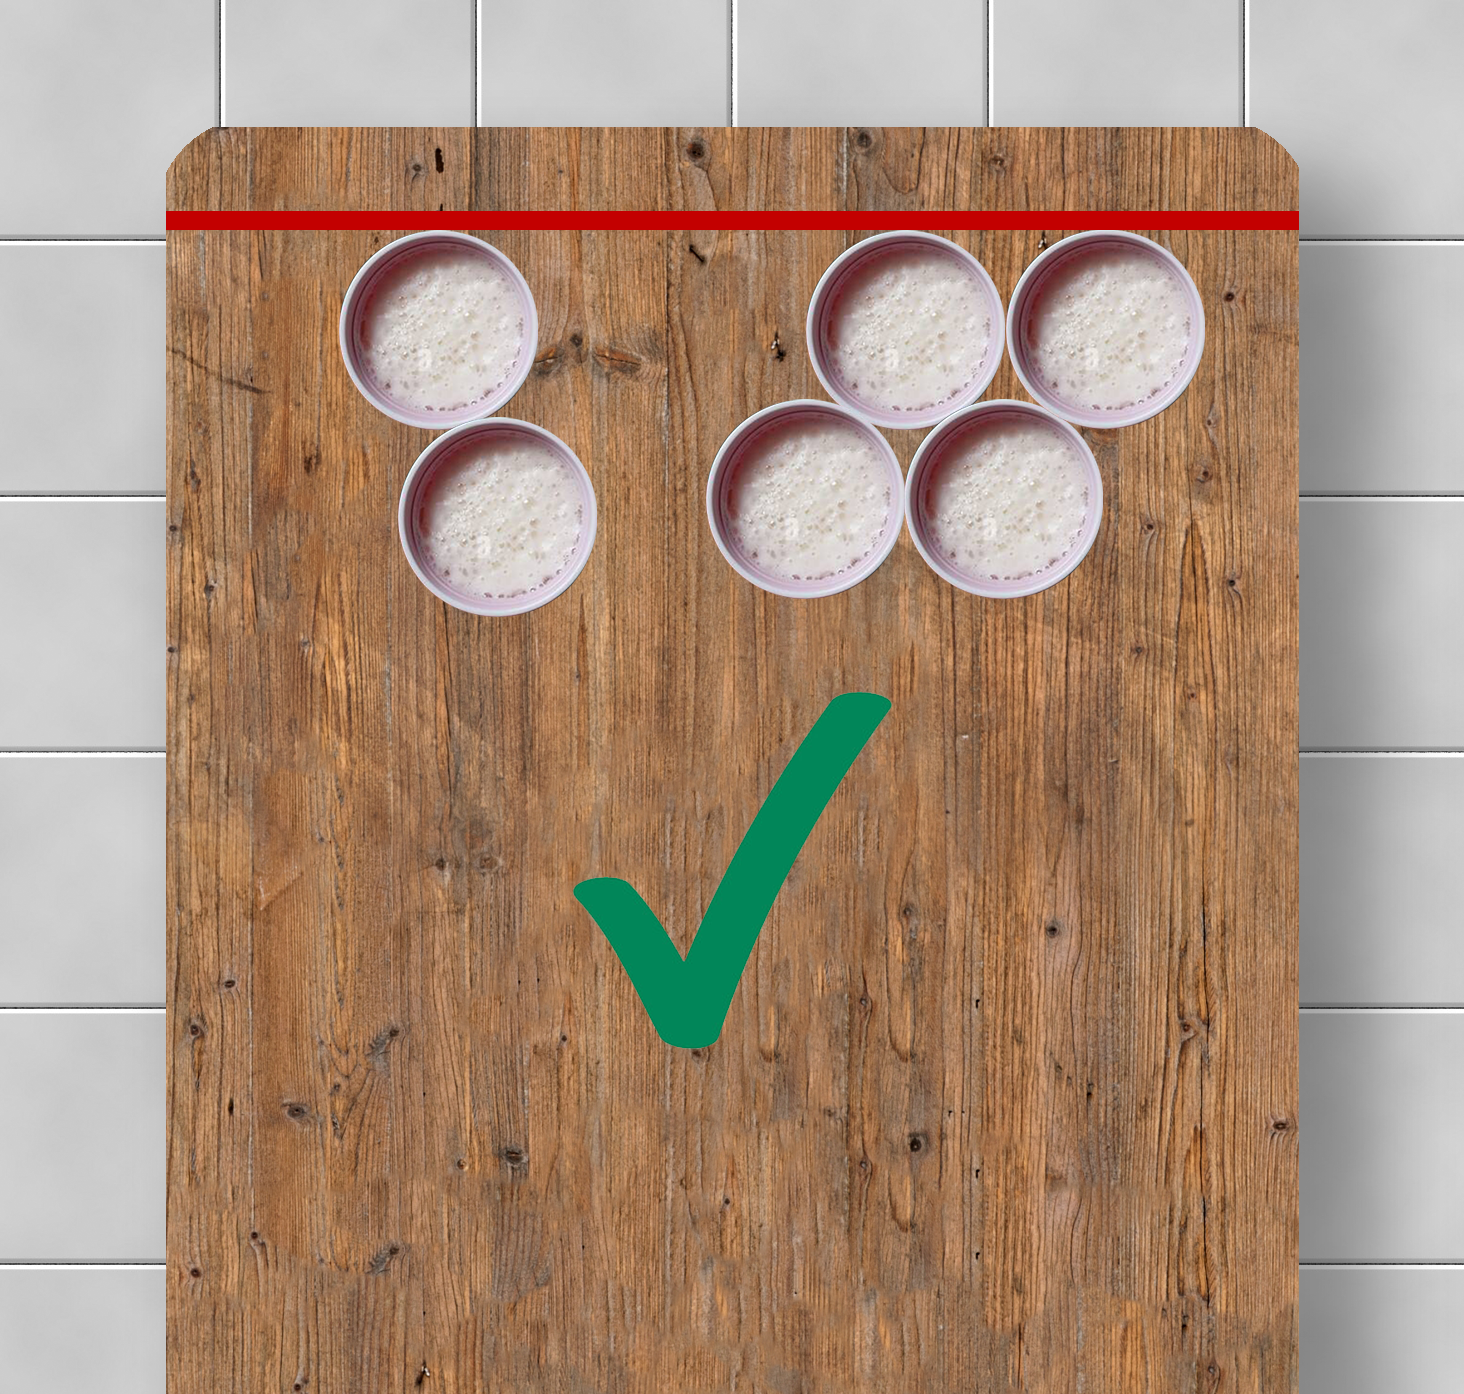
\includegraphics[width=\textwidth]{yes1}
         \caption{erlaubte Formation}
     \end{subfigure}
        \caption{Beispiele zu den Stellungen}
        \label{fig:three graphs}
\end{figure}
\item
    Centern: \\\\
    Wenn die Gegner nur noch einen Becher haben darf man fordern, dass die Gegner ihn auf die Center Position (siehe Abbildung \ref{fig:three graphs}) stellen. 
\end{enumerate}
Nach der Umstellphase ist das selbe Team mit der regulären Wurfphase an der Reihe
\subsubsection{Reguläre Wurfphase} \label{subsub:reguläreWurfphase}
Beide Spielerinnen eines Teams dürfen nacheinander, oder gleichzeitig, ganz wie sie wollen, einen Standardwurf durchführen.\\\\ Nach diesen beiden Würfen ist dasselbe Team mit der BallsBackphase an der Reihe.
\subsubsection{BallsBackphase}\label{subsub:ballsbackphase}
\begin{enumerate}[(1)]
    \item Startbedingungen:\\\\
    In der letzten BallsBackphase oder Regulären Wurfphase haben beide Spielerinnen getroffen.
    \item Ausführung:\\\\
    Beide Spielerinnen dürfen einen Standardwurf werfen\\
Nach diesen beiden Würfen ist die BallsBackphase vorbei und es werden die Startbedingungen für den erneuten Start der BallsBackphase überprüft. Sind diese nicht erfüllt, ist das selbe Team mit der OnFirephase an der Reihe.

\end{enumerate}
\subsubsection{OnFirephase}\label{subsub:onfirephase}
\begin{enumerate} [(1)]
    \item Startbedingungen:\\\\
    Startbedingungen: Mindestens eine Spielerin des Teams, das an der Reihe ist, hat 3 OnFire-Stacks. (siehe Abschnitt \ref{sub:onfirestacks})
    \item Ausführung:\\\\
    Eine der Spielerinnen mit 3 OnFire-Stacks darf 
 einen Standardwurf werfen. Wenn beide Spielerinnen eines Teams 3 Stacks haben, dann wirft diejenige, die als letztes geworfen hat. \\
Nach dem einen Wurf ist die OnFirephase vorbei und es werden die Startbedingungen für eine erneute OnFirephase überprüft. Sind diese nicht erfüllt, geht es mit der Trickshotphase weiter. Sollten sie erfüllt sein, beginnt die OnFirephase erneut.


\end{enumerate}
\subsubsection{Trickshotphase}\label{subsub:Trickshotphase}
\begin{enumerate} [(1)]
    \item Startbedingungen:\\\\
    Das Team an der Reihe hat mindestens einen Trickshot Stack. (siehe Abschnitt \ref{sub:trickshotstackss})
    \item Ausführung:\\\\
    Ein Team wirft so viele Trickshots, wie sie Trickshot Stacks haben. Dabei wechseln sich die beiden Teammitglieder mit dem Werfen immer ab. Dann endet die Trickshotphase. \\\\
\end{enumerate}
Nach dem Ende der Trickshotphase ist das andere Team mit der Umstellphase an der Reihe.
\subsection{Spielende}\label{sub:spielende}
Das Spiel ist vorbei, wenn eine der folgenden beiden Bedingungen eintritt:
\begin{enumerate}[(1)]
    \item Der letzte Becher eines Teams wird als gehitted markiert und sie schaffen keinen Konter (siehe Abschnitt \ref{sec:redemption}).
    \item Es werden bei einer Bemängelung mehr als 80 ml in einem Becher festgestellt (siehe Abschnitt \ref{sec:80ml}).
    \item Es wird ein Deathcup getroffen (siehe Abschnitt \ref{sec:deathcup}).
\end{enumerate}
Die nachfolgenden Punkte werden in beliebiger Reihenfolge nach dem Ende des Spiels abgearbeitet.
\subsubsection{Übrige Becher trinken}\label{subsub:übrigebechertrinken}
Das Verliererteam muss die Becher, die bei dem Gewinnerteam noch auf dem Tisch stehen trinken. Hierbei können ihnen andere Leute, oder auch das Gewinnerteam aus Gnade helfen.
\subsubsection{Nackte Meile}\label{subsub:nacktemeile}
Trifft eine Spielerin im ganzen Spiel keinen einzigen Becher, dann muss sie eine nackte Meile laufen. Ein Treffer in einen eigenen Becher, oder bei Eye to Eye reicht nicht, um die nackte Meile zu vermeiden.\\
Die Route der nackten Meile ist wie folgt:\\
Start an der Wohnungstür der Wal-WG\texttrademark. Dann die Treppe runter, zur Haustür raus, einmal um die Feuerschale im oberen Garten, wieder zur Haustür rein, die Treppe bis ganz oben und wieder runter in die Wal-WG\texttrademark.\\
Im Idealfall läuft man ganz nackt. Aber wenn man es ganz nackt nicht machen würde, kann man auch einzelne Kleidungsstücke anlassen.\\
Wenn mehrere Spielerinnen eine nackte Meile laufen müssen, dann müssen sie das Hand in Hand tun. 

\subsubsection{Foto}\label{subsub:foto}
Von dem Gewinnerteam muss ein Foto gemacht werden. Dieses wird dann entweder an ein Wal-WG\texttrademark-Mitglied geschickt, oder bei dem QR-Code hier/an der Wand hochgeladen.\\ 
\begin{figure}[htbt]
    \centering
    \includegraphics[scale = 0.1]{bilder}
    \caption{Foto Upload}
    \label{fig:fotoupload}
\end{figure}
\chapter{Weitere Regeln}\label{chap:weitereregeln}
Im folgenden Kapitel werden alle weiteren Regeln aufgeführt, nach denen gespielt wird. Sind Regeln hier nicht aufgeführt, so wird auch nicht nach ihnen gespielt.
\section{Bombe}\label{sec:bombe}
Treffen beide Spielerinnen eines Teams in der selben Runde in den selben Becher, werden zusätzlich zu diesem noch 2 weitere als gehitted markiert. Welche die beiden weiteren sind, entscheidet das Team, dessen Becher es sind. \\\\
Wenn das Gegnerteam am Anfang der jeweiligen Phase 4 oder weniger Becher hat, dann zählt nur ein weiterer Becher als gehitted. (Wenn nur noch ein Becher da ist, dann kann dieser auch als doppelt gehitted zählen)\\\\
Um Bomben nicht im Weg zu stehen zählt es zu den guten Manieren, einen Ball, nachdem er in einen Becher geworfen wurde, herauszuholen, bevor der nächste Wurf geworfen wird.
\section{Ellenbogen}\label{sec:ellenbogen}
Wenn eine Spielerin einen Standardwurf ausführt, muss im Moment, in dem der Ball die Hand verlässt, der Ellenbogen hinter ihrer eigenen kurzen Tischkante sein.\\
Das Gegnerteam ist dafür verantwortlich darauf zu achten, dass sich an die Regel gehalten wird. Wenn sie den Verdacht haben, dass der Ellenbogen zu weit vorne war, dann wird ausdiskutiert, ob es tatsächlich so war, wenn es der Fall ist, dann ist der Wurf ungültig und wird nicht wiederholt. Bei einer umstrittenen Entscheidung kann der Wurf auch wiederholt werden.

\section{Redemption}\label{sec:redemption}
Wenn ein Team den letzten Becher $n$ mal als gehitted markiert, muss das andere Team versuchen zu kontern. Dafür starten sie ganz normal in der Umstellphase. Jetzt sammeln sie über alle Phasen Hits. Dann gibt es mehrere Fälle:
\begin{enumerate}[(1)]
    \item Genau $n$ Hits: Konter erfolgreich, es bleiben alle Becher am Tisch genauso stehen
    \item Mehr als $n$ Hits: Konter erfolgreich, alle Hits, die nach dem n-ten Hit passieren zählen ganz regulär
    \item Weniger als $n$ Hits: Konter nicht erfolgreich, das Spiel ist verloren
\end{enumerate}
Spezialfall:\\\\
Team A hat noch einen Becher auf ihrer Seite. Sie sammeln Hits auf alle Becher von Team B. Team B schafft den Konter mit gleich vielen Hits, also Fall (1).\\
Dann gibt es eine Verlängerung. Das heißt, dass beide Teams ihren jeweiligen letzten Becher trinken müssen. Dann stellt jedes Team 3 neue Becher in einer kleinen Pyramide auf, die eine Seite zentriert an der Grundlinie hat und befüllt sie mit der Hälfte der Menge, mit der am Anfang die 10 Becher befüllt wurden. Jetzt wird erneut ermittelt wer anfängt. (siehe Abschnitt \ref{sec:entscheidenweranfängt})\\\\
Verständnishilfe: Eigentlich geht das aus dem oben Geschriebenen eindeutig hervor, trotzdem kam die Frage auf, was passiert, wenn beim Spiel ein Becher gegen einen Becher zuerst getroffen wird, dann aber öfter gekontert wird, als für eine Verlängerung benötigt. Man könnte meinen, dass man Hits mit in die Verlängerung nehmen kann. Dem ist nicht so. Wer den Absatz zum Spezialfall genau lese, dem falle auf, dass der Spezialfall nur eintritt, wenn genau gekontert wird. In unserem Beispielszenario sind wir also in Fall (2). Das Team, dass zuerst den letzten Becher getroffen hat, muss also jetzt kontern. 

\section{Aufsetzer}\label{sec:aufsetzer}
Wenn ein Standardwurf, nachdem er die Hand verlassen hat zuerst den Tisch berührt und dann trifft, dann zählt zusätzlich zum getroffenen Becher noch ein weiterer Becher als gehitted. Welcher dies ist, entscheidet das Team, das ihn trinken muss. Sobald der Ball einmal aufgesetzt hat, darf das Gegnerteam ihn wegschlagen.\\\\
Diese Regel gilt nur, wenn das Gegnerteam am Anfang der jeweiligen Phase noch 5 oder mehr Becher hat.

\section{Deathcup}\label{sec:deathcup}
Wenn ein Becher, den eine Spielerin gerade trinken muss, getroffen wird, dann hat sein Team sofort verloren, außer:\\
Das Gegnerteam muss aus irgendwelchen Gründen keine, oder nicht alle dem Spiel zugehörigen Becher trinken (z.B weil sie Wasser in den Bechern haben und aus der Flasche trinken).
\section{Island}\label{sec:island}
Jeder Spielerin hat einmal im Spiel das Recht Island zu callen. Dazu muss sie eine beliebige Insel nennen. Auch Kontinente zählen als Insel. Dies geht nur, wenn die Gegner am Beginn dieser Wurfphase noch 5 oder mehr Becher hatten. Dann muss sie einen alleinstehenden Becher bestimmen. Als alleinstehend gilt jeder Becher, in der aktuellen Aufstellung keinen Nachbarn mehr hat. Becher, die sich etwas verschoben haben zählen trotzdem noch als Nachbarn. Wenn sie ihren darauffolgenden Wurf in diesen Becher trifft, dann zählt dieser Becher als gehitted und zusätzlich noch ein weiterer. Welcher dies ist, darf das Team, das ihn trinken muss, entscheiden.\\
Wird allerdings ein anderer Becher getroffen, gilt dieser nicht als getroffen. (Dies gilt insbesondere auch bei einem Deathcup (siehe Abschnitt \ref{sec:deathcup}).
\section{Letzter}\label{sec:letzter}
Damit der letzte Becher als gehitted zählt muss er getroffen werden. 
\section{Bitchcup}\label{sec:bitchcup}
Diese Regel fängt mit der ersten Wurfphase an in Kraft zu treten.\\Trifft eine Spielerin den ersten Treffer ihres Teams in einen Bitchcup (siehe Abschnitt \ref{fig:spielaufbau}), muss sie die Hose aus oder komplett herunterziehen, das ist ihre Wahl (wenn sie keine Hose trägt, dann muss das jeweilige Kleidungsstück, das die oberste Schicht der Beinbekleidung darstellt, ausgezogen werden). Sie darf die Hose, oder was auch immer sie ausgezogen hat, wieder anziehen, sobald sie den nächsten Becher der Gegner trifft. \\
Diese Regel ist ähnlich wie die nackte Meile (siehe Abschnitt \ref{sec:nacktemeile}) als keine unbedingte Pflicht zu verstehen, wenn es jemandem unangenehm ist sich auszuziehen, dann muss sie das nicht zwingend tun.\\\\
Wenn am Ende des Spiels eine Hose immer noch unten ist, muss sie unten bleiben bis in einem folgenden Spiel ein Becher getroffen wird. Wenn in diesem folgendem Spiel wieder der Bitchcup getroffen wird, muss die oberste Kleidungsschicht am Oberkörper abgelegt werden. Auch diese Entkleidung ist keine unbedingte Pflicht.\\
Sollte beim Treffen des Bitchcups die Werferin bereits nackt sein, ist er dazu angehalten eine spontane Tanzeinlage zu performen.
\section{Fingern/Blasen}\label{sec:fingern/blasen}
Wenn ein Becher getroffen wird kann der Wurf nicht dadurch ungültig gemacht werden, den Ball herauszufingern oder zu blasen.
\section{80ml}\label{sec:80ml}
Jede Spielerin hat zu jedem Zeitpunkt die Möglichkeit den Füllstand eines noch nicht getrunkenen/nicht gerade getrunken werdenden Bechers des Gegnerteams anzuzweifeln. Dies geht nur bei Bechern, aus denen keine Füllung ungewollt ausgetreten ist. Wenn sich nach einer Messung herausstellt, dass im Becher weniger als 80ml waren, dann muss er getrunken werden. Wenn allerdings 80ml oder mehr drin waren, dann hat das Team des Zweiflers sofort verloren. Diese Überprüfung wird mit der Wal-WG\texttrademark eigenen Bierpongwaage durchgeführt. Das Leergewicht eines Bechers ist:
\section{Weltraumlaser}\label{sec:weltraumlaser}
Jede, die einen Weltraumlaser trifft, bekommt ein eigenes Bild an der Wand. \\\\ Ein Weltraumlaser ist ein von der Fensterseite aus geworfener Ball, der mit viel Wucht gegen die obere Türkante geworfen wird, von der er dann so abspringt, dass er direkt in die Becher der Türseite fliegt. 
\section{Ball im Flug berühren}\label{sec:ballimflugberühren}
Wenn eine Spielerin beim Wurf des Gegners den Ball in der Luft berührt, und der Ball dann keinen Treffer zur Folge hat, dann muss ihr Team einen Becher trinken, welchen sie selbst aussuchen, wenn die beiden folgenden Bedingungen erfüllt sind:
\begin{enumerate}[(1)]
    \item Der Wurf war grob auf Kurs einen Becher zu treffen.
    \item Das Gegnerteam hat nicht einen normalen Wurf und einen Aufsetzer gleichzeitig geworfen.
\end{enumerate}

Sonderfall: \\Der berührte Ball wurde auf nur einen Becher geworfen:\\
	Da der letzte Becher immer getroffen werden muss kann er nicht als Bestrafung getrunken werden müssen. Daher bekommt das Gegnerteam zwei zusätzliche Standardwürfe zugesprochen. 
Außerdem gilt es als Unsportlichkeit und kann zur Disqualifikation führen, vor allem wenn der Wurf auf einem guten Kurs war.

\section{Communitycup}\label{sec:communitycup}
Wenn ein Ball auf irgendeine Art und Weise, aber nicht absichtlich, in einen der leeren Becher kommt, die am Tischrand stehen, dann müssen alle Zuschauerinnen einen Schluck aus ihrem Getränk nehmen.
\section{Becher vorstellen}\label{sec:bechervorstellen}
Um dem entgegenzuwirken, dass ständig Becher am Boden liegen, hat jedes Team das Recht, seine Becher, die nah an der Kante stehen, so weit vorzuschieben, dass sie die Grundlinie noch berühren. 
Das darf man immer, außer wenn ein Gegner gerade schon in der Wurfbewegung ist. 

\section{Becher berühren}\label{sec:becherberühren}
Wenn man nicht eine der folgenden Tätigkeiten ausführt, darf im Spiel kein nicht leerer Becher berührt werden:
\begin{enumerate} [(1)]
    \item Umstellen (siehe Abschnitt \ref{subsub:umstellphase})
    \item Vorschieben (siehe Abschnitt \ref{sec:bechervorstellen})
    \item Ball aus einem Becher herausnehmen
    \item Trinken (siehe Abschnitt \ref{sec:bechertrinken})
    \item Becher der vom Tisch fällt fangen oder wieder aufstellen (siehe Abschnitt \ref{sec:treffer}))
    \item Die Pyramide für die Verlängerung stellen und auffüllen
    
\end{enumerate}
Wenn man dies doch tut, und es war ein eigener Becher, dann muss man ihn trinken. Wenn es ein Becher des Gegnerteams war, dann muss man einen selbstgewählten eigenen Becher trinken. 
\section{Airball}\label{sec:Airball}
Wenn ein Standardwurf weder die Tischplatte, noch irgendetwas anderes auf dem Tisch befindliches berührt, bevor ihn eine gegnerische Spielerin berührt, zählt er als Airball. Hierbei ist dringend \ref{sec:ballimflugberühren} zu beachten. 
\section{Stacks}\label{sec:stacks}
Stacks können von einer Spielerin, bzw. einem Team gesammelt werden. Es gibt drei verschiedene Arten von Stacks, die Trickshot Stacks, die OnFire-Stacks und die OnIce-Stacks.
\subsection{Trickshot Stacks}\label{sub:trickshotstacks}
Wenn eine Spielerin einen Airball wirft, gibt es zwei Optionen:
\begin{enumerate} [(1)]
    \item Das Gegnerteam bekommt einen Trickshot Stack.
    \item Beide Teams einigen sich darauf aufzuheben. Das geht nur, wenn das Werferteam schon mindestens einen Trickshot Stack hat. Bei dieser Option verliert das Werferteam einen Trickshot Stack und das Gegnerteam bekommt für diesen Airball keinen zugesprochen. 
\end{enumerate}
Nach dem Ende der Trickshotphase eines Teams werden dessen Trickhot stacks auf 0 gesetzt
\subsection{OnFire-Stacks}\label{sub:onfirestacks}
Für jeden getroffenen Standardwurf und jeden getroffenen Trickshot bekommt eine Spielerin einen OnFire-Stack(Beim \textit{ Eye to Eye} treffen bringt keinen OnFire-Stack). Trifft sie einen Wurf in der regulären Wurfphase oder in der OnFirephase nicht, werden ihre OnFire-Stacks wieder auf Null gesetzt.
\subsection{OnIce-Stacks}\label{sub:onicestacks}
Für jeden Airball bekommt eine Spielerin einen OnIce-Stack dazu. Die OnIce-Stacks einer Spielerin werden auf Null zurückgesetzt, wenn entweder ein Standardwurf/Trickshot kein Airball ist, oder ein Nervenberuhigungsbecher (siehe \ref{sec:Nervenberuhigungsbecher}) getrunken wird. 
\section{Nervenberuhigungsbecher}\label{sec:Nervenberuhigungsbecher}
Wenn eine Spielerin Drei OnIce-Stacks hat, muss sie einen Becher Wasser zur Nervenberuhigung trinken. Dann werden die OnIce-Stacks wieder auf Null zurückgesetzt.
\section{Behinderung}\label{sec:behinderung}
Es ist verboten, die Gegnerin physisch beim Wurf zu behindern. 
\section{Ball auf Becher}\label{sec:aufbecher}
\subsection{liegen bleiben}\label{sub:liegenbleiben}
Wenn bei einem Standardwurf oder Trickshot der Ball auf den Bechern eines Teams liegen bleibt, ohne hineinzufallen, dann zählt das als ein getroffener Becher. Das Team, bei dem er liegt, darf sich aussuchen, welcher Becher als getroffen zählt.
\subsection{springen}\label{sub:springen}
Springt ein Ball auf den Bechern/dem Becher eines Teams, darf dieses ihn ohne Konsequenzen wegschlagen. Diese Regel zählt stärker als \ref{sec:ballimflugberühren}.
\appendix
\part {Anhang} \label{part:anhang}
\chapter{Patchnotes}\label{chap:patchnotes}
\chapter[Abbildungsverzeichnis]{Abbildungs- verzeichnis}\label{chap:Abbildungsverzeichnis}
\listoffigures
\chapter[Anträge auf Regeländerungen]{Anträge auf Regel- änderungen}\label{chap:antrageaufregelanderung}
 Auf den folgenden Seiten ist Platz für Anträge auf Regeländerung. Bitte beschreibe genau, was wie und warum geändert werden soll.\\ \newpage
 \newgeometry{total = {4in, 7in}}
\neueregel
\neueregel
\neueregel
\neueregel
\neueregel
\neueregel
\neueregel
\neueregel
\neueregel
\neueregel
\neueregel
\neueregel
\neueregel
\restoregeometry
\chapter{RegelPDF}\label{regelpdf}
Wenn du großer WalWG\texttrademark Bierpong Anwalt werden willst kannst du hier das PDF des Regelwerks herunterladen:
\begin{figure}
    \centering
    
\includegraphics[scale = 0.1]{Bierpongregeln}
    \caption{RegelPDF}
\end{figure}

\end {document}